\documentclass[a4paper,12pt]{article}
\usepackage[utf8]{inputenc}
\usepackage{graphicx}
\usepackage{tabularx}
\graphicspath{../images}
\usepackage{minted}
\usepackage[a4paper,width=150mm,top=25mm,bottom=30mm,bindingoffset=6mm]{geometry}
\graphicspath{{../images}}
\usepackage{float}
\usepackage{wrapfig}
\usepackage{natbib}
\usepackage{ifplatform}
\usepackage[nottoc]{tocbibind}
\bibliographystyle{agsm}
\title{EPQ Product Written Report: Building a 32-bit Operating System}
\date{12th December 2024} 
\begin{document}
\begin{titlepage}
\maketitle
%\tableofcontents
 \abstract{
An operating system (OS) is a collection of programs that provide basic, low-level features required for a computer. An OS has several key features \citep{igcse_textbook}:
\begin{itemize}
\item Providing a hardware-agnostic application interface
\item Managing resources and processes
\item Providing a basic user interface
\item Enforcing process security and isolation
\end{itemize}
OSes communicate with hardware, software, and the user and manage computer resources to effectively perform these tasks(see fig \ref{fig:osschematic}). Due to their requirements, Operating systems are extremely complex, and have grown in size over time to support increasingly complex hardware . For example, the Linux Kernel has grown from around 10243 LoC (lines of code) to $\geq 37$ million LoC in version 6.11-rc4 (counted by me using \texttt{cloc}). The size can make OS development daunting to new systems programmers. 

In this project, I aim to develop a basic operating system subset for IBM PC-like designs supporting modern processor features like Protected mode, virtual memory, paging, and modern executable interfaces. In doing this, I aim to improve my own skills in programming without abstraction and my understanding of Data Structures \& Algorithms. 
}
\end{titlepage}
% \tableofcontents
\section{Introduction}
An operating system (OS) is a collection of programs that provide basic, low-level features required for a computer. An OS has several key features \citep{igcse_textbook}:
\begin{itemize}
\item Providing a hardware-agnostic application interface
\item Managing resources and processes
\item Providing a basic user interface
\item Enforcing process security and isolation
\end{itemize}

\begin{wrapfigure}{r}{0.5\textwidth}
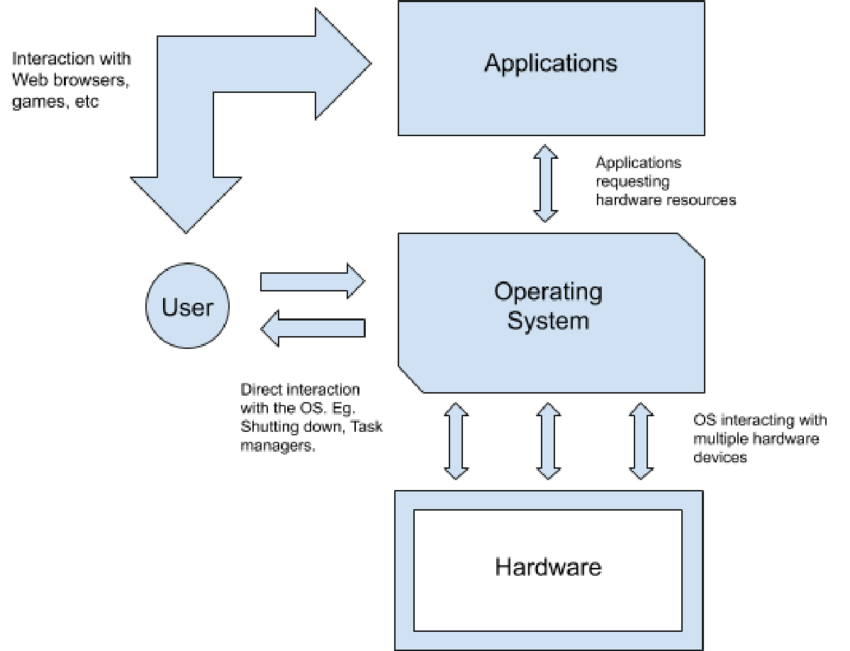
\includegraphics[width=0.48\textwidth]{osschematic}
\caption{High-level block diagram of an operating system} 
\label{fig:osschematic}
\end{wrapfigure}

OSes communicate with hardware, software, and the user and manage computer resources to effectively perform these tasks(see fig \ref{fig:osschematic}).

Due to their requirements, Operating systems are extremely complex, and have grown in size over time to support increasingly complex hardware . For example, the Linux Kernel has grown from around 10243 LoC (lines of code) to $\geq 37$ million LoC in version 6.11-rc4 (counted by me using \texttt{cloc}). The size can make OS development daunting to new systems programmers. 

My interest in operating systems comes primarily from my own experience in configuring them and tinkering with the internals of modern releases of Linux and FreeBSD, both common operating systems. Changing settings and tracking the impact on performance got me interested in OS development. I aimed to write a simple operating system which used a subset of the features I was tweaking on my own system. 
\section{Aims} 
\begin{enumerate}
\item To write a basic OS subset targeted towards IBM PC-like designs.
\item To build my skills in programming without abstraction (close to hardware)
\item To improve my Data Structures \& Algorithms skills 
\end{enumerate}
\section{Research} 

\subsection{Initial Reading}

The IGCSE textbook taught me the basics of the Von Neumann model, which is the computing model applied in almost all modern processors, including the \texttt{i386}  \citep{igcse_textbook}.

Other resources that proved vital as I was beginning my research included the OSDev Wiki \citep{osdev-wiki}. The authority and accuracy of this source were occasionally dubious; however, the "Further Reading" sections and citations were excellent for gathering further sources. 

\subsection{Further Reading}

I found two excellent sources of information on the \texttt{i386} processor. The first of these two is Ralf Brown's Interrupt List \citep{rbil}, which exhaustively detailed the IBM PC's behaviour. This, in conjunction with Intel's official datasheets for the \texttt{i386} \citep{i386_datasheet}, made up most of my further reading about the \texttt{i386}. 

Where the \texttt{i386} reference was cumbersome e.g. when looking up single instructions / condition codes, the x86 and amd64 Instruction Reference \citep{x86_reference} was invaluable. It is a script-separated version of the Intel official reference, and was an enormous time-saver when checking simple condition codes. 

For other peripherial chips, I used official datasheets from their respective suppliers, like the PS/2 datasheet from Altium \citep{ps2_reference}, and the the \texttt{i8259} datasheet available from Intel \citep{i8259_datasheet}. 

\subsection{Primary Research - Existing Artefact Analysis}

I chose to include artefact analysis after finding valuable pointers in source code for my project. One of the sources I looked over was MikeOS \citep{mikeos}, a simple real-mode (16-bit) operating system.


The other operating system I looked at was Linux; the codebase often contained helpful pointers to the bugs in my own code in the form of comments. Linux is the world's most popular operating system today, so looking at its \texttt{0.01} release was a valuable source of information \citep{linux}. Though the comments contained profane language, this did not significantly impact the credibility of the source as it is the world's most popular operating system \citep{linux_adoption}. 

Overall, my primary research was useful as it included real code that provided me with valuable pointers (but not solutions) to the problems I was facing. 

\subsection{Source Testing}
I made sure to test the quality of every source by evaluating its currency, relevance, authorship, accuracy, and purpose. I have included a few examples of these tests below: \\
\subsubsection{\texttt{i386} Reference}
\begin{tabularx}{\textwidth}{l|X|l}
Criterion & Evaluation & Score \\
\hline
Currency & The source was published in 1987 - not very recent. & 4/10 \\
Relevance & The source is expressly for systems/application developers - extremely relevant. & 9/10 \\
Accuracy & The source is extremely accurate, with few known errata. & 9/10 \\
Authority & The source is published by the manufacturers/designers of the chip. The source is an official document. The author is trustworthy. & 9/10 \\
Purpose & To introduce programmers to the \texttt{i386}, which was new at the time. & 9/10 \\
\end{tabularx}
\bigskip

This source scores 40/50 on the CRAAP test, and is extremely reliable. This was an example of an extremely high-quality source.\\
\subsubsection{OSDev Wiki}
\begin{tabularx}{\textwidth}{l|X|l}
Criterion & Evaluation  & Score \\
\hline
Currency & The source is updated frequently; very recent. & 8/10 \\
Relevance & The source is expressly for operating system development - extremely relevant. & 9/10 \\
Accuracy & The source had a few errors.  & 4/10 \\
Authority & The source is published by anonymous authors. & 3/10 \\
Purpose & To support developers in writing Operating systems. & 8/10 \\
\end{tabularx}
\bigskip

This source scores 32/50 on the CRAAP test. It is an average quality source, but still useful.
\section{Planning}
\begin{figure}[H]
		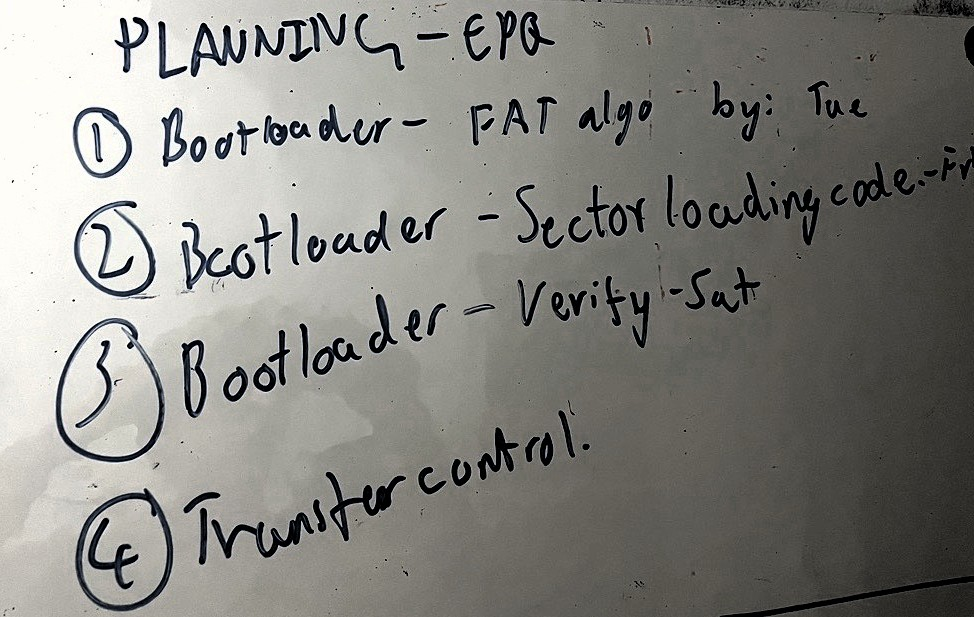
\includegraphics[width=\textwidth]{planning}
\caption{My initial planning method}
\end{figure}

Pre-MPR, my planning method was slightly rudimentary. I detailed a high-level plan in the production log, and then split the tasks up into several sub-tasks of manageable size (around 1 day's worth of work). I then wrote 6-7 subtasks per week on a whiteboard and then struck them off as I achieved the milestones. I then erased the whiteboard at the end of the week and wrote the next few subtasks. \\

\begin{figure}
		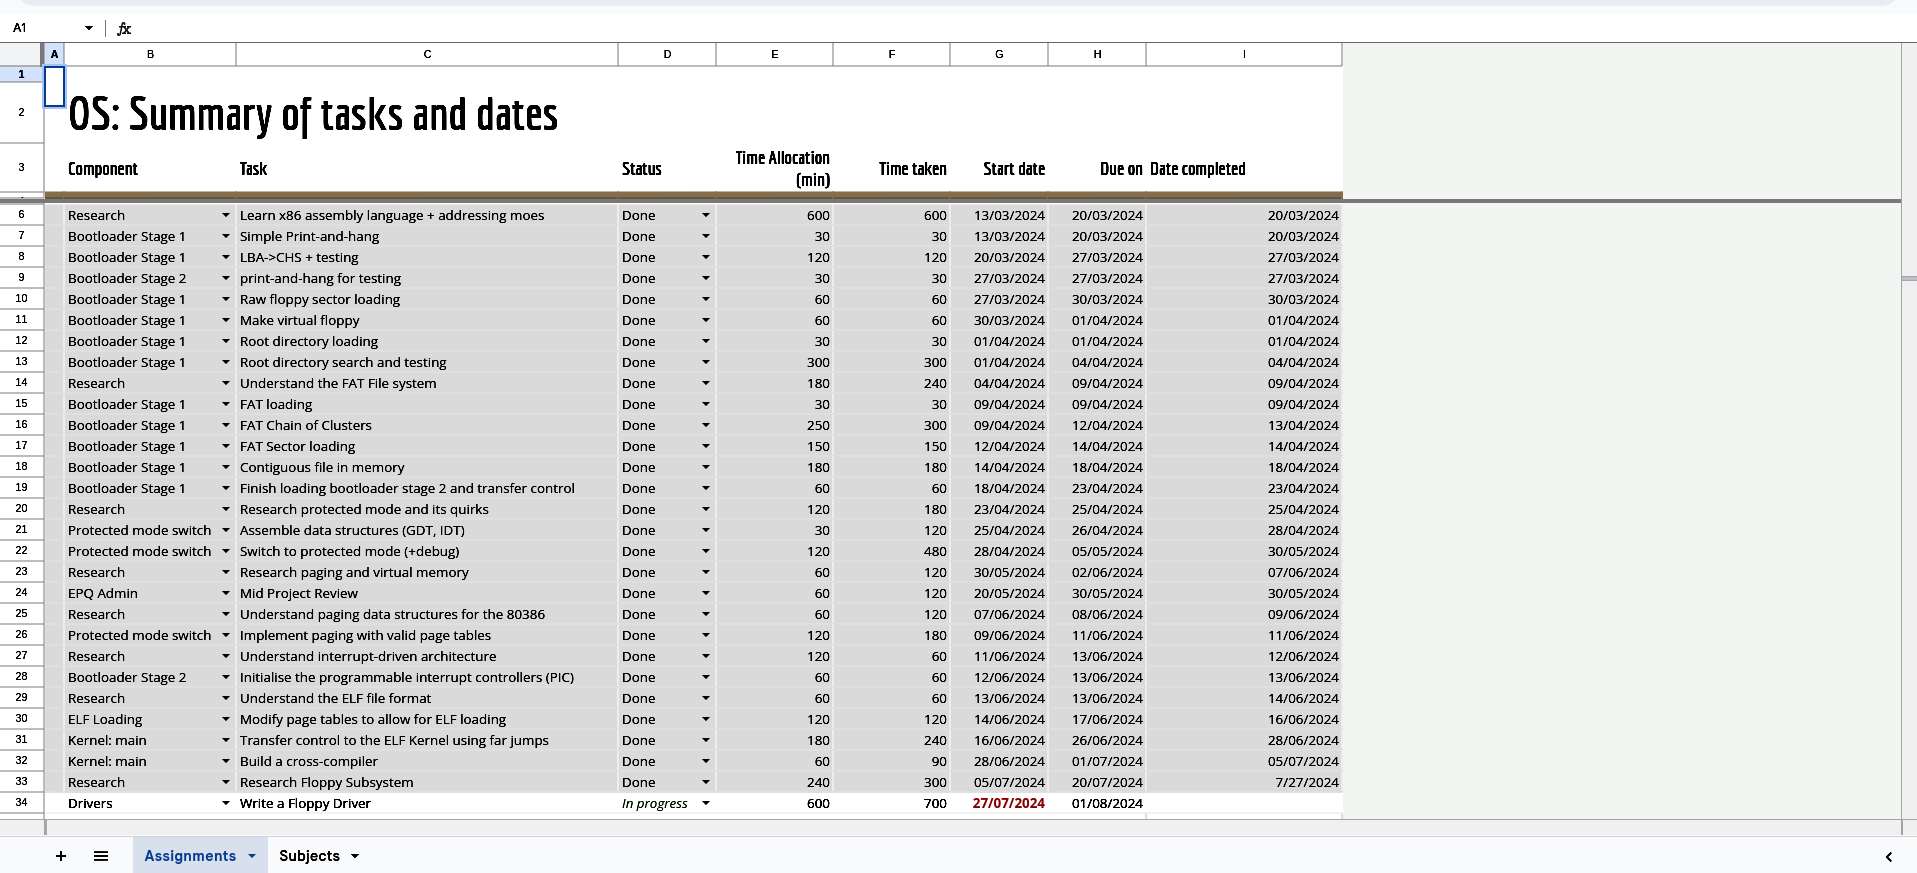
\includegraphics[width=\textwidth]{plan-spreadsheet}
		\caption{Planning method post-MPR - visualisation in Fig. \ref{fig:gantt}}
\end{figure}
\begin{figure}\label{fig:gantt}
	\includegraphics[width=\textwidth]{gantt}
	\caption{A Gantt chart of my plans (the blank spaces are for AS-levels and a separate research project)}
\end{figure}

This planning method was not particularly effective for the EPQ as there was no record of my progress. Post-MPR, however, I switched to using a spreadsheet to track my progress. This had several advantages, as I could categorize my work into different classes, record dates when work was completed, and keep track of how closely I was adhering to my plan.

\section{Operating System Development}

\subsection{Booting}
\subsubsection{1st stage bootloader}
\begin{listing}[H]
\ifwindows
\inputminted[breaklines, linenos, numbersep=5pt, firstline=11,lastline=37]{nasm}{../os/kernel/boot/mbr.asm} % ugly hack but whatever
\else
\inputminted[breaklines, linenos, numbersep=5pt, firstline=11,lastline=37]{nasm}{/home/vedantg/os/kernel/boot/mbr.asm} % ugly hack but whatever
\fi
\caption{The standardised data structures in the MBR, required to read or write from the disk}
\label{listing:mbr}
\end{listing}

Bootloaders take the form of 512 raw bytes written to the first 512 bytes on the disk, a region termed the Master Boot Record. This section of the disk has a specified format. 

After this table is the beginning of the bootloader, whose task it is to read the floppy and load the rest of the operating system into memory. Given that the above table takes up around 40 bytes, only 480 bytes remain for the bootloader, which means the bootloader must be small. 
Since a large quantity of hardware must be initialised to use protected mode. I used a second-stage bootloader to initialise the processor and peripherals.
\subsubsection{2nd stage bootloader}
I used this stage to initialise only the CPU and prepare it to run the kernel, which was entirely 32-bit in nature. This meant I simply loaded the kernel into memory, and then started fully initialising the processor's different modes, continuing the booting process.
\begin{listing}[H]
\ifwindows
\inputminted[breaklines, linenos, numbersep=5pt, firstline=338, lastline=342]{nasm}{../os/kernel/boot/stage2.asm} % ugly hack but whatever
\else
\inputminted[breaklines, linenos, numbersep=5pt, firstline=338, lastline=342]{nasm}{/home/vedantg/os/kernel/boot/stage2.asm} % ugly hack but whatever
\fi
\caption{The 2nd stage bootloader transferring control to the kernel at the end of its execution}
\label{listing:stage2}
\end{listing}

I used the 2nd stage bootloader to switch the processor from operating in 16-bit real mode (its initial state) to 32-bit protected mode. I then initialised memory by writing page tables, and initialised paging (a memory-managing technique). I also initialised the interrupts subsystem, which allows the processor to handle peripheral communications, loaded and interpreted the kernel, and transferred control over to it.
\subsection{Kernel}
\begin{listing}[H]
\ifwindows
\inputminted[breaklines, linenos, numbersep=5pt, firstline=35, lastline=53]{c}{../os/kernel/main.c} % ugly hack but whatever
\else
\inputminted[breaklines, linenos, numbersep=5pt, firstline=35, lastline=53]{c}{/home/vedantg/os/kernel/main.c} % ugly hack but whatever
\fi
\caption{The main kernel file that receives control from the 2nd stage bootloader}
\label{listing:kernel}
\end{listing}
The kernel is the core of the operating system, and manages memory, disk access, processes, CPU time, and peripherals. Developing a kernel is key to operating system development, but it is also the portion that takes the most technical skill, as correctly interfacing with peripherals is difficult. The initial pre- Mid Project Review scope of my EPQ involved developing a full kernel, with process management, but I reduced the scope of my project to include only hardware and memory management due to difficulties with implementation.
\subsubsection{Interrupts}
Interrupts from hardware / peripherals are handled by two chips termed ``Programmable Interrupt Controllers''. These chips are fairly easy to program, and once set up along with the corresponding memory structures, pass on hardware interrupts and exceptions to the operating system. These chips were set up alongside the interrupt memory structures in the 2nd stage bootloader, and required only installation of interrupt handlers that were part of the kernel.
\begin{listing}[H]
\ifwindows
\inputminted[breaklines, linenos, numbersep=5pt, firstline=37, lastline=46]{c}{../os/kernel/arch/i386/interrupts.c} % ugly hack but whatever
\else
\inputminted[breaklines, linenos, numbersep=5pt, firstline=37, lastline=46]{c}{/home/vedantg/os/kernel/arch/i386/interrupts.c} % ugly hack but whatever
\fi
\caption{The default interrupt handler, which is replaced by other interrupt handlers}
\label{listing:interrupts}
\end{listing}

\subsubsection{Keyboard Driver}
Developing the keyboard driver was relatively painless. Keyboards send scancodes to their host computer along with an interrupt indicating a scancode is available to be read, which provide information about which key is pressed when. The keyboard driver handles the interrupt and gets the scancodes, interprets the scancodes according to the keymap in force, and passes on the characters and key combinations to the operating system. 

\begin{listing}[H]
\ifwindows
\inputminted[breaklines, linenos, numbersep=5pt, firstline=10, lastline=55]{gas}{/home/vedantg/os/kernel/hw/i8042/i8042_isr.s} % ugly hack but whatever
\else
\inputminted[breaklines, linenos, numbersep=5pt, firstline=10, lastline=55]{gas}{/home/vedantg/os/kernel/hw/i8042/i8042_isr.s} % ugly hack but whatever
\fi
\caption{The Keyboard interrupt handler}
\label{listing:keyboard}
\end{listing}

One problem I faced was not fully understanding the documentation detailing the chip's behaviour. An interrupt is raised every time a byte needs to be passed, which means that multiple interrupts can be raised for the same key-down or key-up event. I wrongly understood the peripheral as sending only one interrupt per key event, but using the debugger for some time helped me find this error and quickly rectify it. 

\subsubsection{VGA}
The VGA driver was also thankfully very simple. In the IBM PC, the VGA framebuffer (a record of every pixel on the display) is memory-mapped to the physical address \texttt{0xB8000}, which means that writing to this location was in effect equivalent to printing on the screen \citep{ibmpc_reference}. A simple memory copy sufficed for these purposes. 
\begin{listing}[H]
\ifwindows
\inputminted[breaklines, linenos, numbersep=5pt, firstline=53, lastline=58]{c}{/home/vedantg/os/kernel/hw/vga/vga.c} % ugly hack but whatever
\else
\inputminted[breaklines, linenos, numbersep=5pt, firstline=53, lastline=58]{c}{/home/vedantg/os/kernel/hw/vga/vga.c} % ugly hack but whatever
\fi
\caption{VGA printing routines}
\label{listing:vga}
\end{listing}

\subsubsection{Floppy}
The floppy driver caused me by far the greatest grief. The 82077A is an extremely complicated chip with a lot of different operating modes, parameters, etc along with a significant list of behaviours deviating from both the specification and information available online \citep{82077a_reference}. This chip was supposed to be used with a DMA (Direct Memory Access) controller, which would essentially allow the CPU to run other tasks while disk I/O occurred in the background. However, the setup of these chips, especially in protected and paged mode, was exceptionally complicated. This driver took up far more time than I was expecting, and it was one of the major reasons why I revised my MPR plan significantly.

\begin{listing}[H]
\ifwindows
\inputminted[breaklines, linenos, numbersep=5pt, firstline=39, lastline=50]{c}{/home/vedantg/os/kernel/hw/i82077a/i82077a.c} % ugly hack but whatever
\else
\inputminted[breaklines, linenos, numbersep=5pt, firstline=39, lastline=50]{c}{/home/vedantg/os/kernel/hw/i82077a/i82077a.c} % ugly hack but whatever
\fi
\caption{Part of the floppy driver containing data structures necessary}
\label{listing:floppy}
\end{listing}



\section{Critical Evaluation}

This task was an exceptionally challenging one for me, and it involved learning a lot of skills, from low-level programming to comprehension of technical references and datasheets. In those ways, I achieved my secondary aims.
My primary aims were not realised to their full extent, however I have written a significant portion of the operating system, and not much more work is necessary to turn it into a full-fledged system. If more time was available to write, I would add in process management as part of the code. The ELF loader is already present, so an executable format is available; logic to parse the filesystem is already written; and all the necessary drivers have been completed, with the exception of the timer (which is a simple chip and will not take much time). 
\bibliography{../references}
\end{document}
